\documentclass{scrartcl}

\usepackage[T1]{fontenc}
\usepackage[utf8]{inputenc}

\title{Mobile Dev 6.1P}
\author{Daniel Coady (102084174)}
\date{13/10/2019}

\usepackage{graphicx}

\begin{document}

\maketitle

\begin{figure}[h]
    \centering
    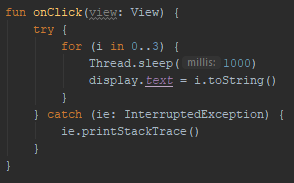
\includegraphics{images/screen1.png}
    \caption{Original code}
\end{figure}
The problem with this original code is that it would hold up the main thread of the
application. Because of this, all other operations were also halted and the application
became completely unresponsive. To fix this we can create an AsyncTask to handle this
operation in the background.

\pagebreak

\begin{figure}[h]
    \centering
    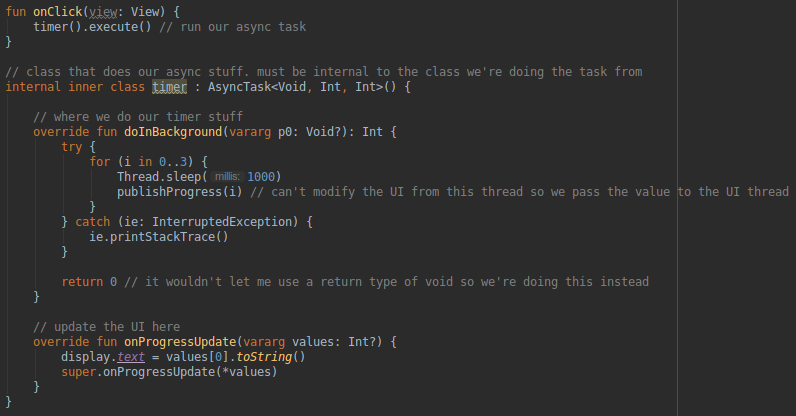
\includegraphics[scale=0.52]{images/screen2.png}
    \caption{New code}
\end{figure}

\section*{How the code works}
\subsection*{onClick()}
When the user clicks the button, we construct a new instance of the timer class and tell
it to execute it's task.

\subsection*{doInBackground()}
This is where the countdown code is placed since anything running here will be run on a
separate thread to the main one, allowing for normal operation to resume even when the
countdown is occuring. There is one change that was made to the code however, and that
is where we change the text inside of our text view. To do this we actually need to
publish that progress has been made so that we may update the UI accordingly. The reason
why this change was made is because the UI may not be modified from outside of the UI thread.

\subsection*{onProgressUpdate()}
Finally here we can update our UI since from within this method we have access to the UI
thread.

\end{document}
